\documentclass{standalone}
\usepackage{tikz,xcolor,amsmath}
\usetikzlibrary{decorations.pathreplacing}
\definecolor{body}{RGB}{50,50,50}
\definecolor{dim}{RGB}{90,90,90}
\definecolor{effectGreen}{RGB}{20,130,20}
\definecolor{effectOrange}{RGB}{180,100,10}
\definecolor{effectBlue}{RGB}{20,80,160}
\begin{document}
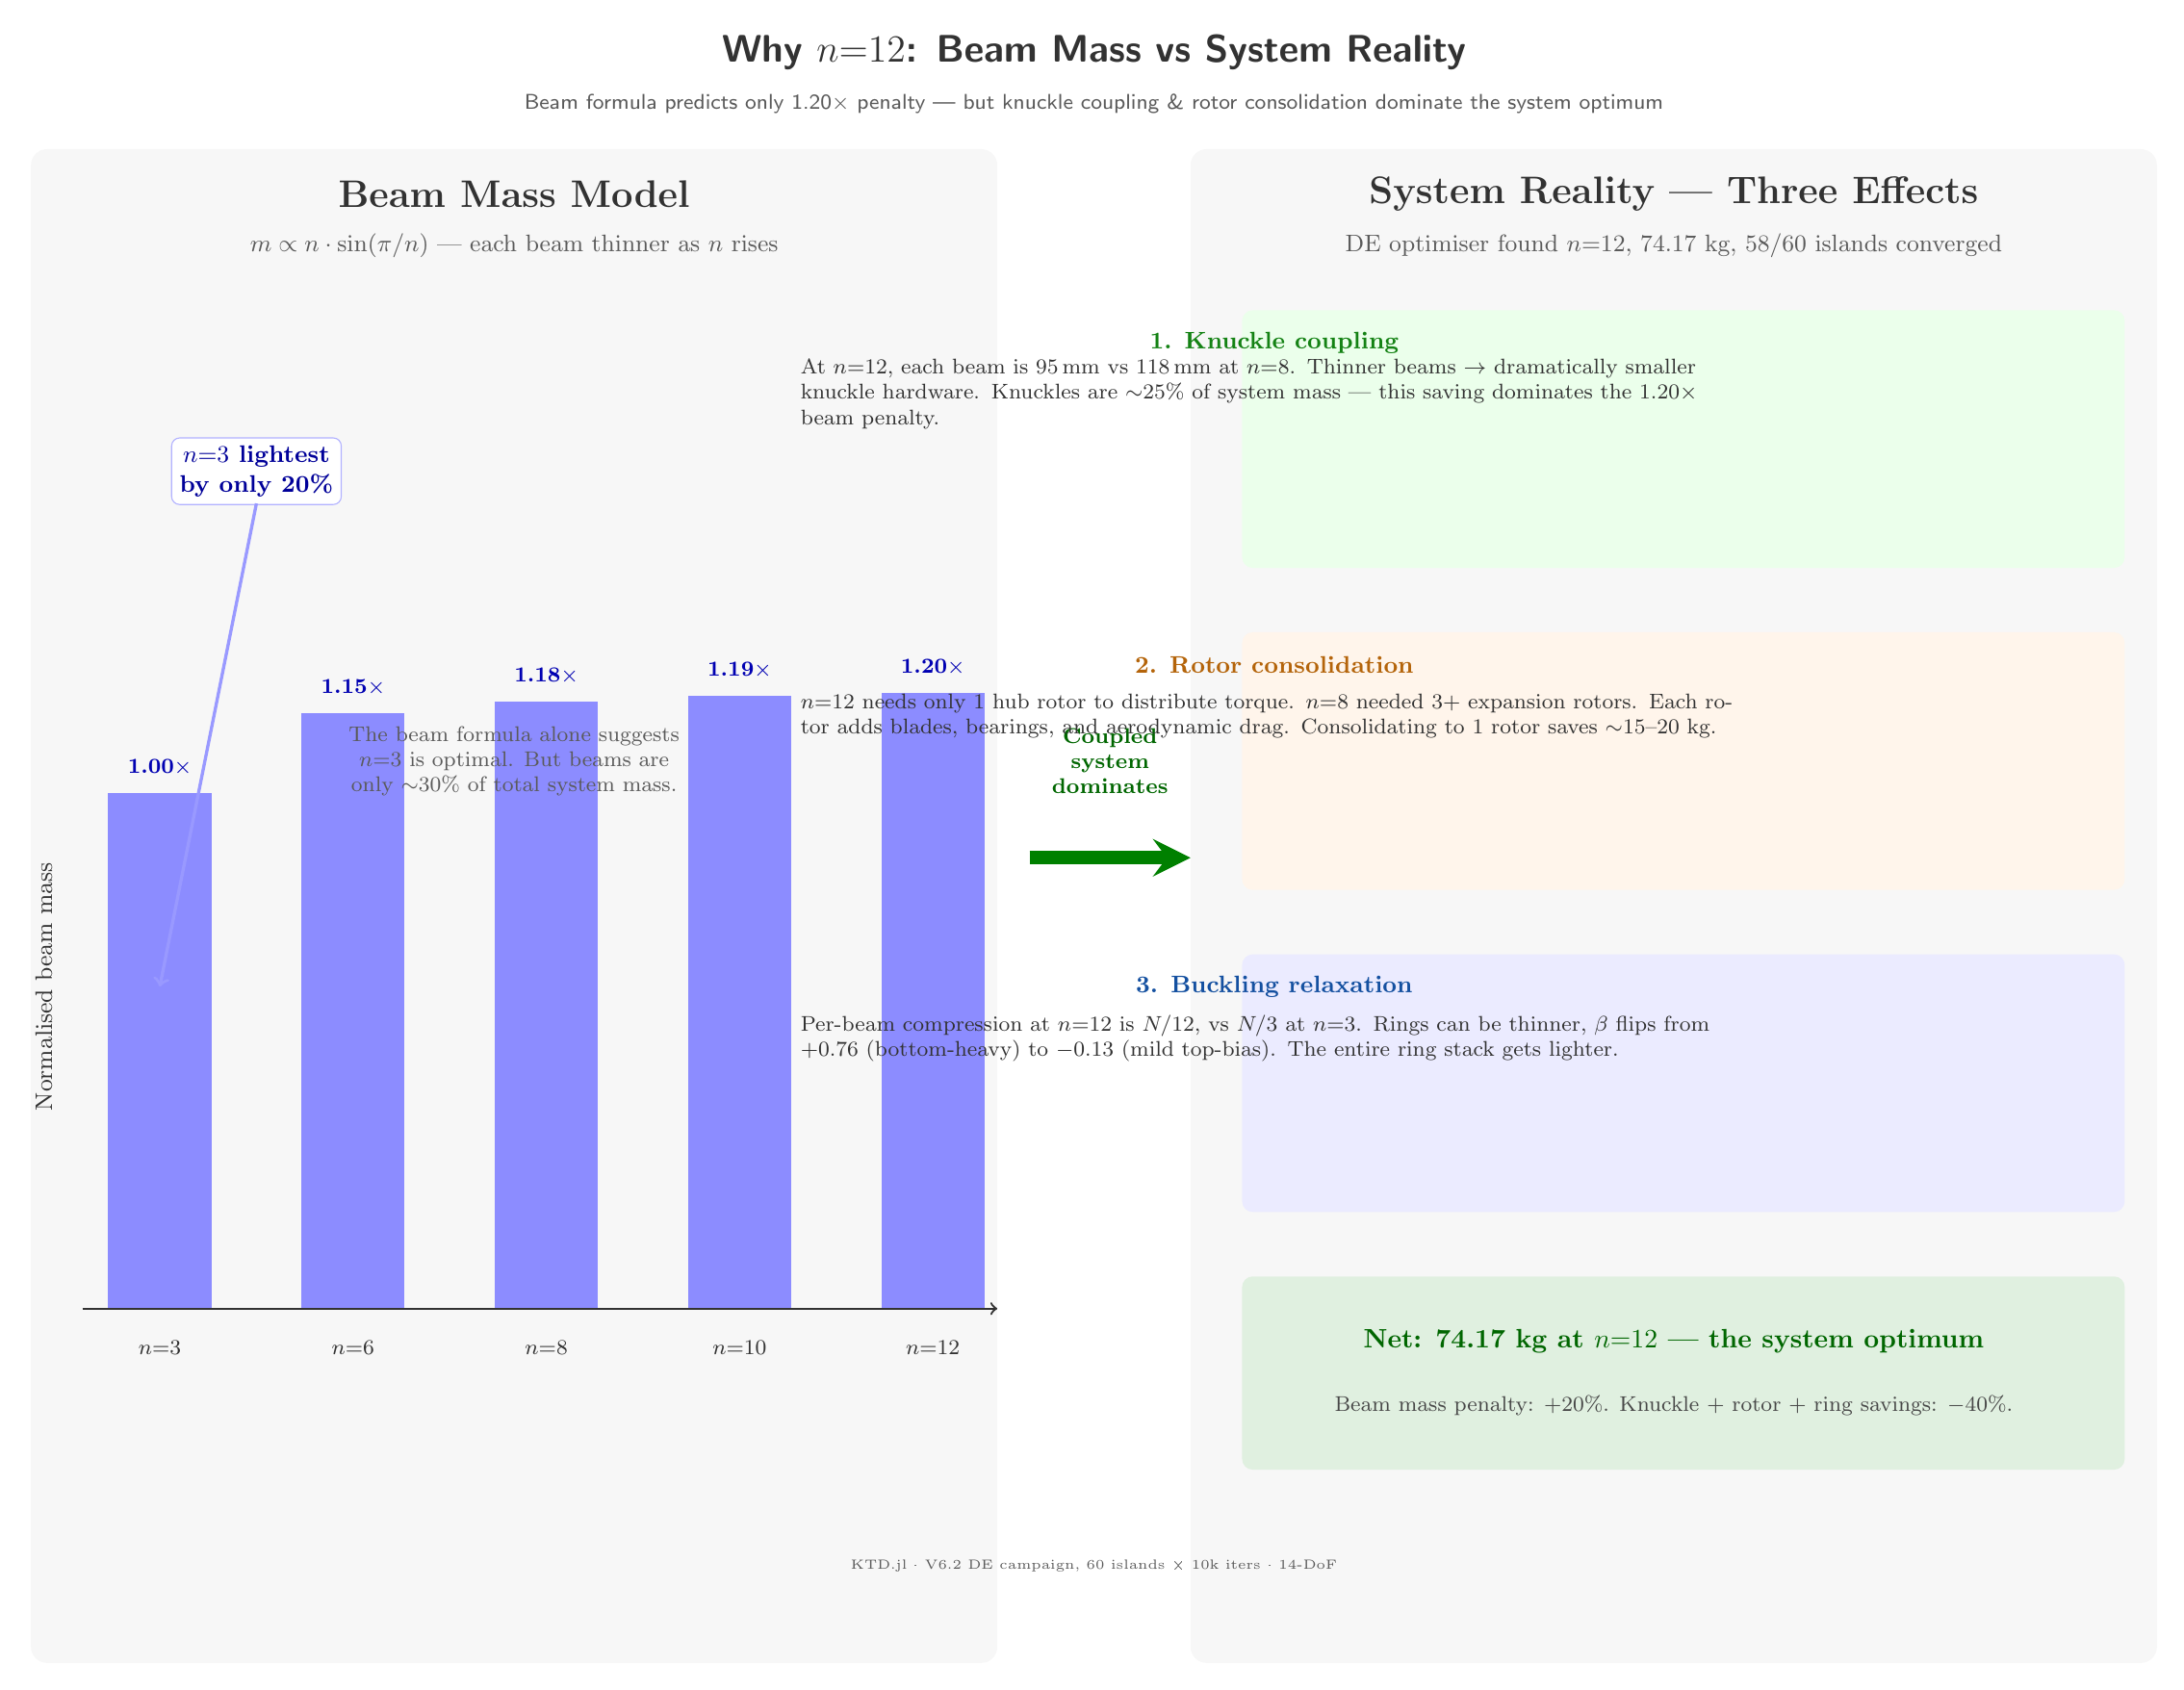
\begin{tikzpicture}[scale=0.85]

% ── Title ──
\node[font=\Large\sffamily\bfseries,body] at (16.0, 22.5) {Why $n{=}12$: Beam Mass vs System Reality};
\node[font=\footnotesize\sffamily,dim] at (16.0, 21.7) {Beam formula predicts only 1.20$\times$ penalty — but knuckle coupling \& rotor consolidation dominate the system optimum};

% ═══════════════════════════════════════════
% PANEL 1: Beam-only mass model
% ═══════════════════════════════════════════
\begin{scope}[shift={(0,0)}]
  \fill[black!3, rounded corners=6pt] (-0.5,-2.5) rectangle (14.5, 21.0);
  \node[font=\bfseries\Large,body] at (7.0, 20.3) {Beam Mass Model};
  \node[font=\small,dim] at (7.0, 19.5) {$m \propto n \cdot \sin(\pi/n)$ — each beam thinner as $n$ rises};

  \foreach \n/\val/\label/\x in {3/1.000/1.00/1.5, 6/1.155/1.15/4.5, 8/1.178/1.18/7.5, 10/1.189/1.19/10.5, 12/1.195/1.20/13.5} {
    \pgfmathsetmacro{\barht}{\val * 8.0}
    \fill[blue!45] ({\x-0.8}, 3.0) rectangle ({\x+0.8}, {3.0+\barht});
    \node[font=\footnotesize\bfseries, blue!70!black] at (\x, {3.0+\barht+0.4}) {\label$\times$};
    \node[font=\footnotesize,body] at (\x, 2.4) {$n{=}\n$};
  }

  \draw[->, thick,body] (0.3, 3.0) -- (14.5, 3.0);
  \node[font=\small,body, rotate=90] at (-0.3, 8.0) {Normalised beam mass};

  \node[font=\small\bfseries, blue!60!black, align=center, fill=white, draw=blue!30, rounded corners=3pt, inner sep=3pt] at (3.0, 16.0) {$n{=}3$ lightest\\by only 20\%};
  \draw[->, blue!40, line width=1.2pt] (3.0, 15.5) -- (1.5, 8.0);

  \node[font=\footnotesize,dim, align=center] at (7.0, 11.5) {The beam formula alone suggests\\$n{=}3$ is optimal. But beams are\\only $\sim$30\% of total system mass.};
\end{scope}

% ── BRIDGE ARROW ──
\draw[->, line width=5pt, >=stealth, green!50!black] (15.0, 10.0) -- (17.5, 10.0);
\node[font=\bfseries\footnotesize, green!40!black, align=center] at (16.25, 11.5) {Coupled\\system\\dominates};

% ═══════════════════════════════════════════
% PANEL 2: System reality
% ═══════════════════════════════════════════
\begin{scope}[shift={(18.0,0)}]
  \fill[black!3, rounded corners=6pt] (-0.5,-2.5) rectangle (14.5, 21.0);
  \node[font=\bfseries\Large,body] at (7.0, 20.3) {System Reality — Three Effects};
  \node[font=\small,dim] at (7.0, 19.5) {DE optimiser found $n{=}12$, 74.17 kg, 58/60 islands converged};

  \fill[green!8, rounded corners=4pt] (0.3, 14.5) rectangle (14.0, 18.5);
  \node[font=\bfseries\small,effectGreen] at (0.8, 18.0) {1. Knuckle coupling};
  \node[font=\footnotesize,body, align=left, text width=12.5cm] at (0.8, 17.2) {At $n{=}12$, each beam is 95\,mm vs 118\,mm at $n{=}8$. Thinner beams $\rightarrow$ dramatically smaller knuckle hardware. Knuckles are $\sim$25\% of system mass — this saving dominates the 1.20$\times$ beam penalty.};

  \fill[orange!8, rounded corners=4pt] (0.3, 9.5) rectangle (14.0, 13.5);
  \node[font=\bfseries\small,effectOrange] at (0.8, 13.0) {2. Rotor consolidation};
  \node[font=\footnotesize,body, align=left, text width=12.5cm] at (0.8, 12.2) {$n{=}12$ needs only 1 hub rotor to distribute torque. $n{=}8$ needed 3+ expansion rotors. Each rotor adds blades, bearings, and aerodynamic drag. Consolidating to 1 rotor saves $\sim$15--20 kg.};

  \fill[blue!8, rounded corners=4pt] (0.3, 4.5) rectangle (14.0, 8.5);
  \node[font=\bfseries\small,effectBlue] at (0.8, 8.0) {3. Buckling relaxation};
  \node[font=\footnotesize,body, align=left, text width=12.5cm] at (0.8, 7.2) {Per-beam compression at $n{=}12$ is $N/12$, vs $N/3$ at $n{=}3$. Rings can be thinner, $\beta$ flips from $+$0.76 (bottom-heavy) to $-$0.13 (mild top-bias). The entire ring stack gets lighter.};

  \fill[green!50!black!12, rounded corners=4pt] (0.3, 0.5) rectangle (14.0, 3.5);
  \node[font=\bfseries,green!40!black] at (7.0, 2.5) {Net: 74.17 kg at $n{=}12$ — the system optimum};
  \node[font=\footnotesize,body!90] at (7.0, 1.5) {Beam mass penalty: $+$20\%. Knuckle + rotor + ring savings: $-$40\%.};
\end{scope}

\node[font=\tiny,dim] at (16.0, -1.0) {KTD.jl · V6.2 DE campaign, 60 islands × 10k iters · 14-DoF};

\end{tikzpicture}
\end{document}
